\begin{figure}
	\begin{center}
		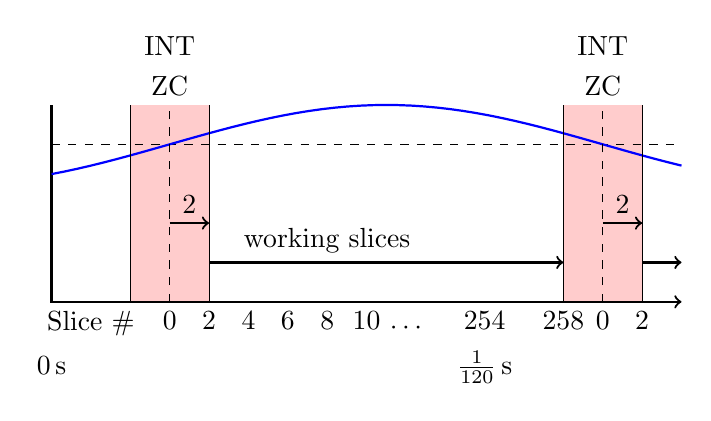
\begin{tikzpicture}[scale=.5]
			\fill [red!20] (2,0) -- (2,5) -- (4,5) -- (4,0) -- cycle;
			\fill [red!20] (13,0) -- (13,5) -- (15,5) -- (15,0) -- cycle;
			\draw [thick, <-] (16,0) -- (0,0) -- (0,5);
%			\draw [thick] (0,5) -- (16,5);
%			\draw [dashed] (8,0) -- (8,10);
%			\draw [dashed] (16,0) -- (16,10);
			\node [below] at (0,-1) {\vphantom{$1\over1$}0\,s};
			\node [below] at (11,-1) {$1\over120$\,s};
			%\node [below] at (16,0) {$1\over60$\,s};
%			\foreach \x in {1, 2, ..., 259} {
%				\draw [very thin] (\x*16/260,2) -- (\x*16/260,8);
%			}

			\draw [dashed] (0,4) -- (16,4);
			\draw [thick,blue] plot[samples=50,domain=0:16](\x,{sin ((\x-3)*(3.1415926/11) r)+4});
			\draw [dashed] (3,0) -- (3,5);
			\draw [dashed] (14,0) -- (14,5);

			\node [below] at (1,0) {Slice \#};
				
			\foreach \x in {0, 2, ..., 10} {
				\node [below] at (\x/2+3,0) {\x};
			}
			\foreach \x/\xx in {11/254, 13/258} {
				\node [below] at (\x,0) {\xx};
			}
			\foreach \x in {0, 2} {
				\node [below] at (\x/2+14,0) {\x};
			}
			\node [below] at (9,0) {\strut$\cdots$};
			\node [above] at (3,5) {ZC};
			\node [above] at (14,5) {ZC};
			\node [above] at (3,6) {INT};
			\node [above] at (14,6) {INT};
			\foreach \x in {2, 4, 13, 15} {
				\draw (\x,0) -- (\x,5);
			}
			\foreach \x in {3, 14} {
				\draw [thick,->] (\x,2) -- (\x+1,2);
				\node [above] at (\x+.5,2) {2};
			}
			\draw [thick,->] (4,1) -- (13,1);
			\draw [thick,->] (15,1) -- (16,1);
			\node [above] at (7,1) {working slices};
		\end{tikzpicture}
		\caption{\label{fig:timingideal}Cycle Timing with No Phase Difference}
	\end{center}
\end{figure}
